\chapter{Conclusion}

\section{Summary}
In this work, a deep learning based open-set logo retrieval framework was introduced, in the scope of sport videos. The task has a lot of challenges, which is due to the often poor visibility of the logos in these videos. The proposed system rests upon proposal based Convolutional Neural Networks. The region proposals are generated by a Faster R-CNN, trained for detecting logos generally. To compare the quality of the proposed system,  a Faster R-CNN is taken as baseline, which generally holds almost state-of-the-art performance on closed-set logo retrieval, evaluated on the test dataset of FlickrLogos-32. The achieved performance of the introduced solution surpasses the baseline method by a large margin.
\section{Future Work}
During this work, it was realized, that the majority of logos in sport videos are text based. This is especially prevalent for videos from small sport events, wherein the advertisements are from local, not so well known companies.
Additionally, one should consider the figure \ref{f:logodetectorfool}, which would very likely fool the proposed logo detector with the sign "TRIBUNA", resulting in a false positive detection.
\begin{figure}
  \centering
  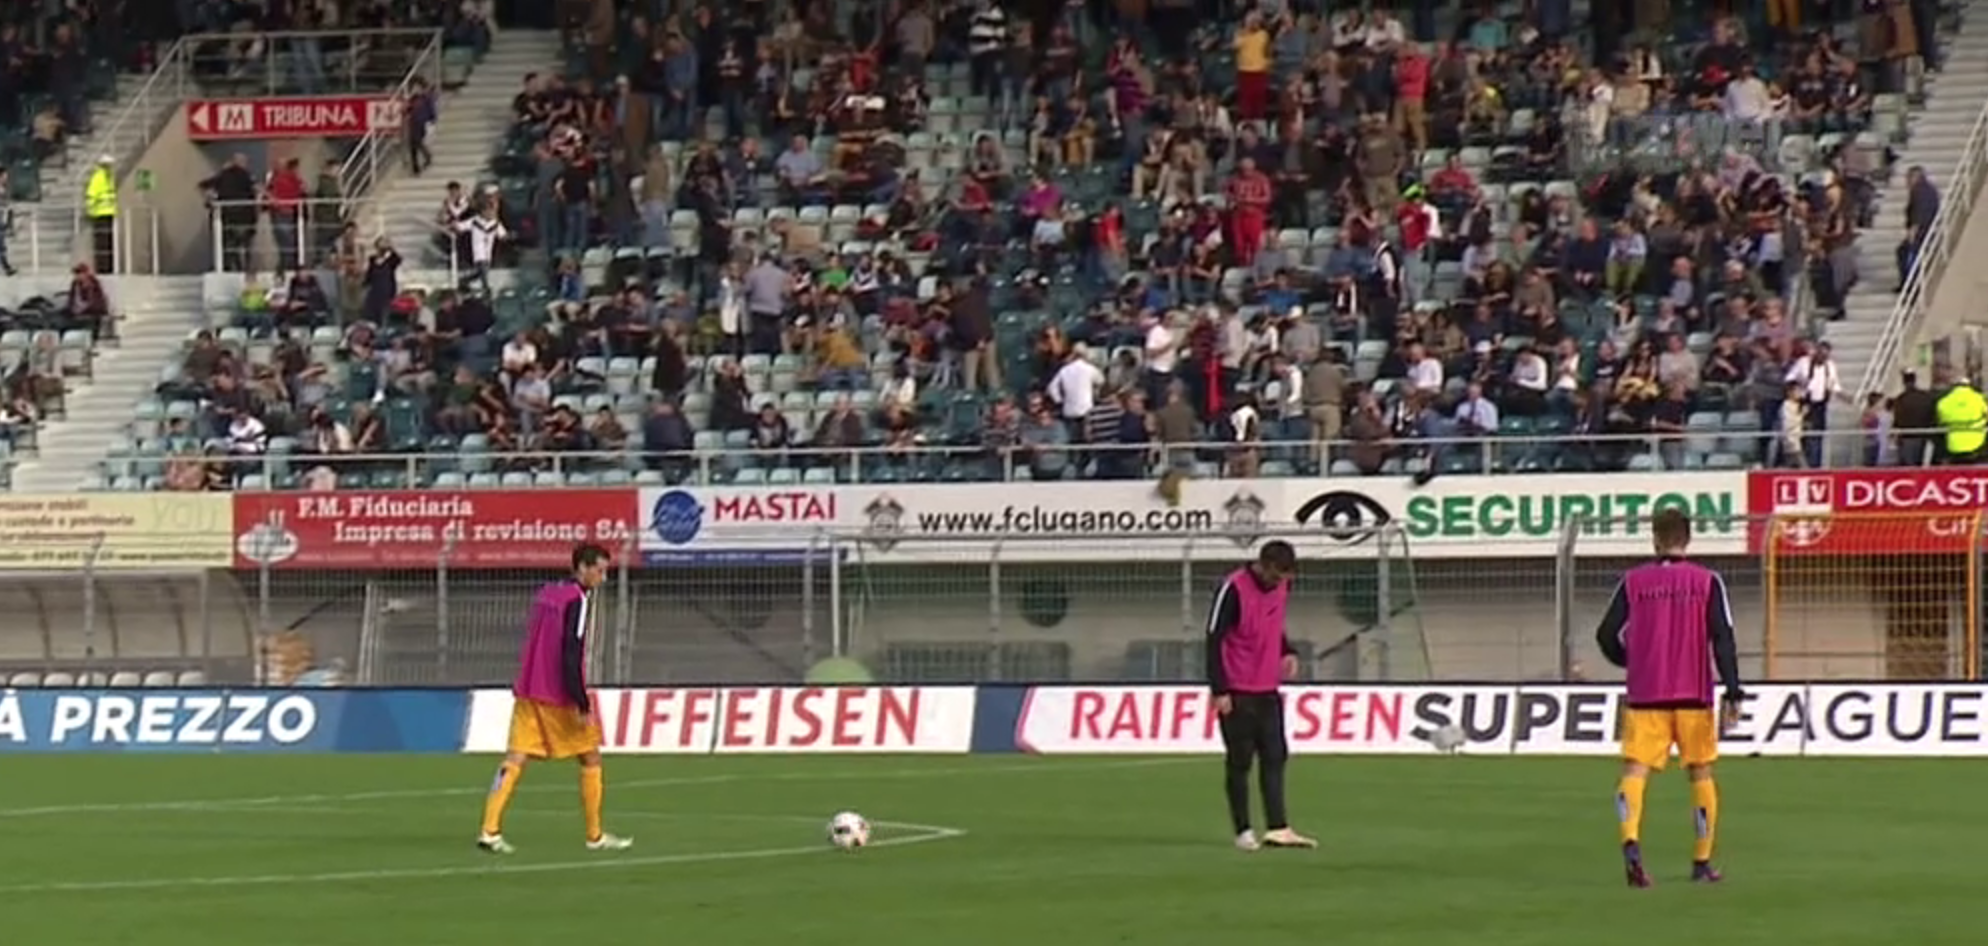
\includegraphics[height=50mm]{images/mt/logodetectorfool.png}
  \caption{A tough example for the logo detector, because of the sign on the top left part of the image}
  \label{f:logodetectorfool}
\end{figure}
For this reason, a logo retrieval system should be extended by a text recognition subsystem e.g. with the work of \cite{Jaderberg14d}. It utilizes synthetic data to train a neural network to recognize words. For unknown words, the system could generate training data, and fine-tune the pre-trained network on demand. For this purpose, the needed computational time should be examined.
However, there are a large number of logos, consisting only of a shape (e.g. Nike, Chanel, Audi, Apple, etc),  and there are font types, differing significantly from the common fonts. These circumstances would make the task of the text recognizer difficult. Therefore, the system should be able to detect and recognize text on the query image, then search for correspondences in the search set only by text recognition or with a combination of convolutional feature similarities as done in this work. The performance of the feature extractor part of the system can be further increased by building an ensemble of them with an appropriate combination.

Maximum Activation of Convolutions (MAC) was successfully used by \cite{DBLP:journals/corr/ToliasSJ15}, \cite{DBLP:journals/corr/AzizpourRSMC14}, \cite{DBLP:journals/corr/RadenovicTC16} for object and scene retrieval. It could be evaluated for logo retrieval too as another feature extraction method.

In order to increase the robustness of the system and reduce the false positive recognitions, the logos, which are detected only for a few frames can be discarded. Additionally, if a logo is recognized many frames in a row, the integration of an object tracking solution could help to identify and fill gap frames, wherein the particular logo is not detected. Such a system could reduce the number of misclassifications further.